\section{Method RQ 1 - Finding the critical factors for walkability}\label{rq1}
\subsection{Literature study}
From literature research, all possible problems that elderly with a rollator can encounter were gathered. Together with the extend of the problem importance. This to form the first main idea of what the possible critical factors could consist of and the eventual list of findings will be used to support and design the interviews with the elderly and finding requirements in the policy and design policies.
The literature study was conducted from October 2014 until January 2015. 

\subsection{Interviews}
In the initial idea was an interview that would consist of 3 parts; first a general part, about age, health and the use of the rollator. The second part is a list of possible problems the participant could encounter. The third part would be drawing on a map, where the participant walks and where certain problems occurred. See overview \ref{interview}. Though after developing and experimenting the final form and the method of conducting changed quickly. 

\begin{figure}[h]
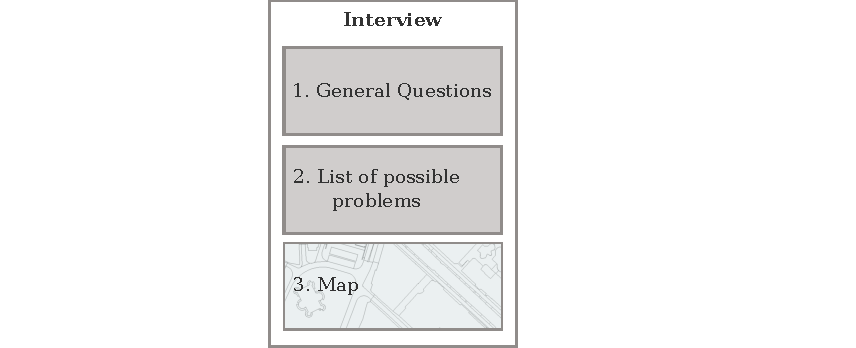
\includegraphics[width=\textwidth]{img/M_interview.pdf}
\centering
\caption{The 3 parts of the interview \label{interview}}
\end{figure}

The questionnaire as shown in Annex \ref{Aquest}, consisting of several pages was developed. The questionnaire was tested, with the researchers grandparents. This concluded that the questionnaire is not a good form for obtaining information form elderly. The reaction of the participants was, that things were unclear and not all questions were answered. Also the amount of text scared the elderly, feeling uncomfortable with their abilities of reading and writing. Therefore, the form of the interview quickly changed to an informal chat, were the researcher used a check-list, making sure all questions were asked while chatting in random order.

The second part, containing a list of possible problems the elderly could encounter was constructed after the literature research. 5 categories are constructed:

\begin{itemize}
\item Quality of the pavement
\item Obstacles
\item Overall business
\item Safety feeling
\item Environmental characteristics
\end{itemize}

The total list can be found in annex \ref{Aelderly}. For the elderly did not feel like reading too much, also this part of the questionnaire was conducted orally. Every possible problem on the list, were read out loud to the elderly and asked to rate from 1 to 5, 1 is they never encounter the problem to 5; they always encounter the problem. The conducting researcher circled the number from 1 till 5 according to the story of the participant. 

The third part, drawing or pointing out problems on a map was quickly cancelled, as the elderly had difficulties reading the maps. They did, though, name streets and locations but the conducting researcher was too unfamiliar with the surroundings to translate this quickly onto the map. 

Several elderly care houses were contacted as well as the neighbourhood care of Amsterdam centre. While sounding enthusiastic from the first point, it was hard to arrange appointments with elderly. 

The total amount of participants for personal interviews were only 2. 

Next to this, also participants on the Rollator Loop were interviewed. Around 10 people were shortly interviewed about the general problems they encounter while walking outdoors. But not the complete list. 
